% Wrapped beside the text when the preamble loads wrapfig (\input it between paragraphs);
% otherwise an ordinary float of the same width.
\ifdefined\wrapfigure
\begin{wrapfigure}{r}{0.5\linewidth}
\vspace{-1em}
\centering
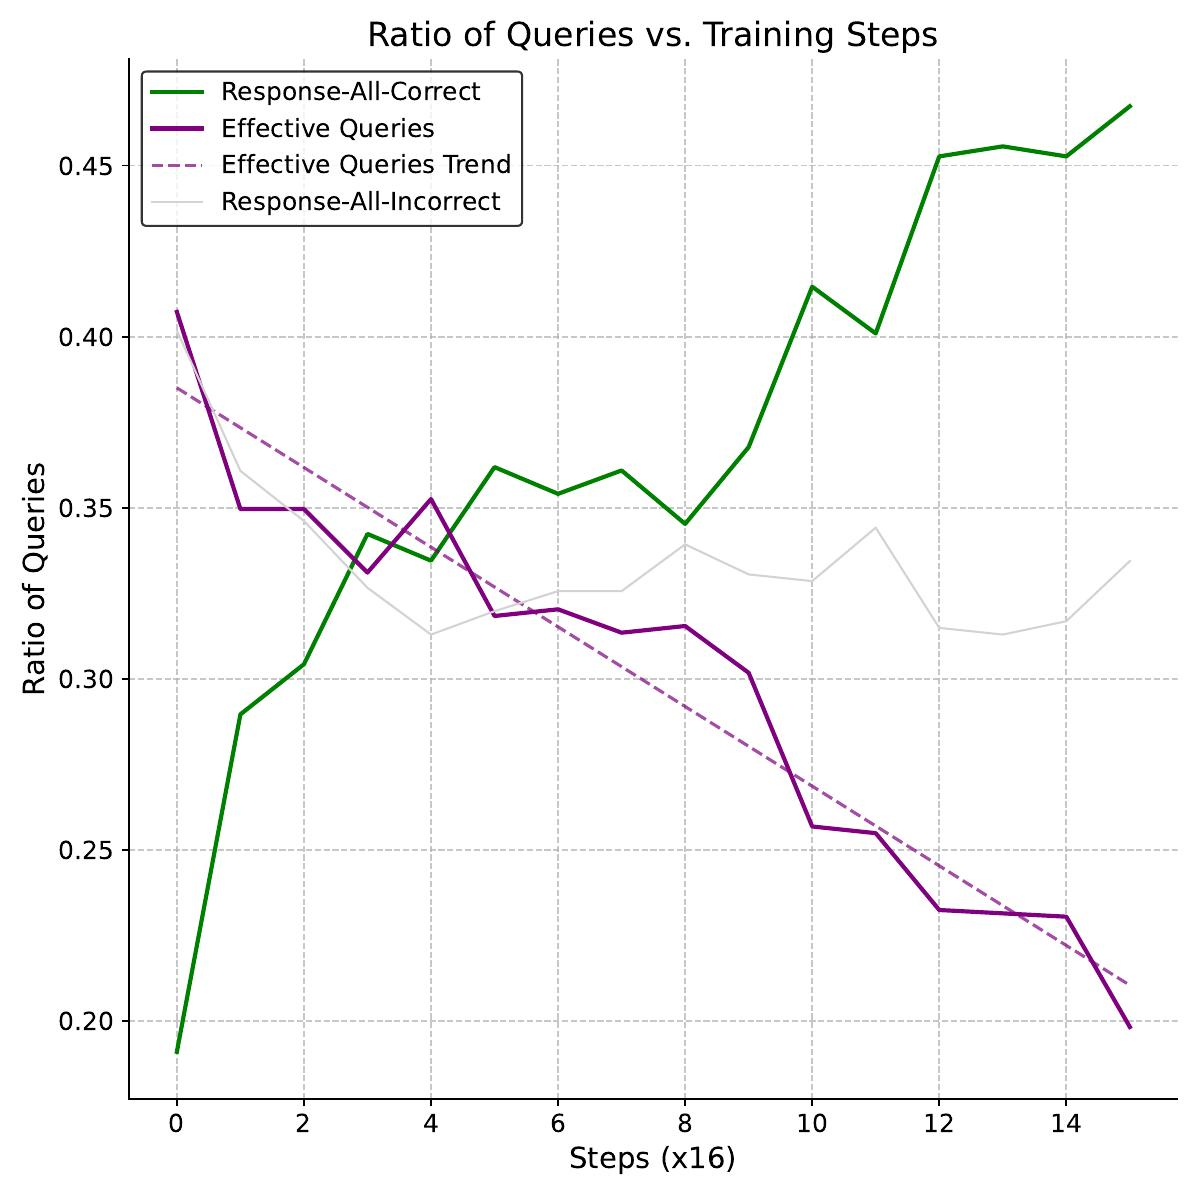
\includegraphics[width=\linewidth]{figures/vanishing_adv.jpg}
\caption{\small \textbf{Vanishing advantages in GRPO training.} Fraction of training queries per step (x-axis: logged points, one every 16 training steps) whose rollouts are all correct (green), all incorrect (gray) or mixed (``effective queries'', purple; dashed: linear trend). Only mixed groups receive a non-zero group-normalised advantage. Over training the effective fraction falls from about 0.41 to 0.20, while the all-correct fraction rises from about 0.19 to 0.47.}
\label{fig:vanishing_adv}
\vspace{-1em}
\end{wrapfigure}
\else
\begin{figure}[tb]
\centering
\begin{minipage}{0.5\linewidth}
\centering
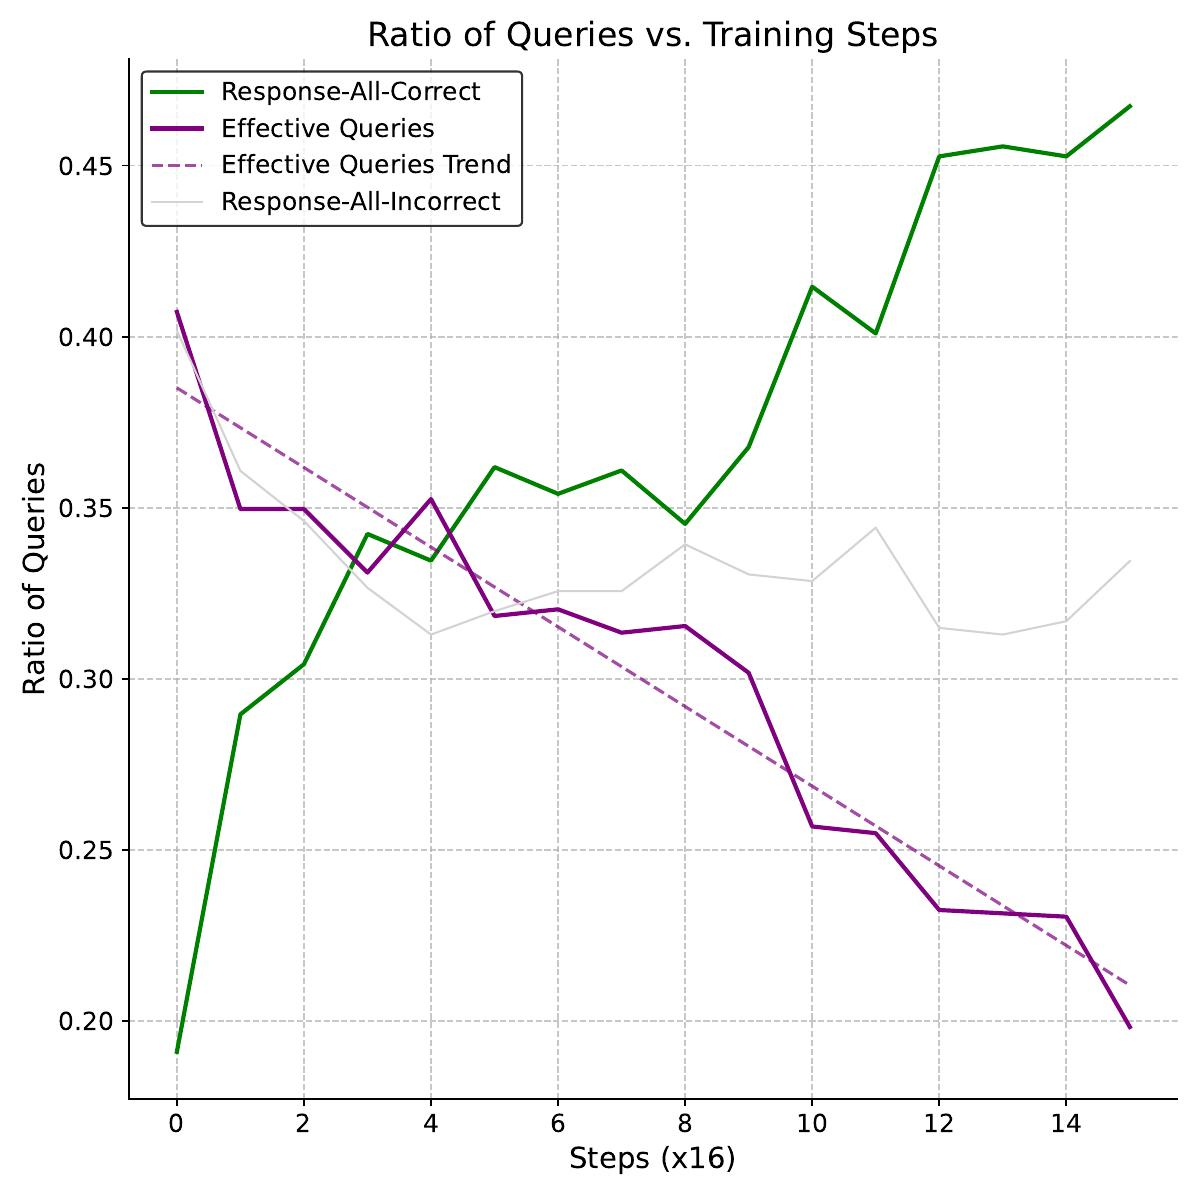
\includegraphics[width=\linewidth]{figures/vanishing_adv.jpg}
\caption{\small \textbf{Vanishing advantages in GRPO training.} Fraction of training queries per step (x-axis: logged points, one every 16 training steps) whose rollouts are all correct (green), all incorrect (gray) or mixed (``effective queries'', purple; dashed: linear trend). Only mixed groups receive a non-zero group-normalised advantage. Over training the effective fraction falls from about 0.41 to 0.20, while the all-correct fraction rises from about 0.19 to 0.47.}
\label{fig:vanishing_adv}
\end{minipage}
\end{figure}
\fi
